\chapter{KIỂM THỬ VÀ ĐÁNH GIÁ HỆ THỐNG}

\section{Mục tiêu và phương pháp kiểm thử}

Mục tiêu của giai đoạn kiểm thử không chỉ dừng lại ở việc đảm bảo các chức năng phần mềm hoạt động đúng theo tài liệu đặc tả SRS (như chức năng Upload, Chat Sandbox), mà quan trọng hơn là đánh giá định lượng chất lượng của hệ thống trí tuệ nhân tạo. Để thực hiện điều này, nhóm đã sử dụng phương pháp kiểm thử tự động thông qua module Benchmark, kết hợp với bộ tiêu chuẩn RAGAS (Retrieval Augmented Generation Assessment) nhằm đo lường hiệu suất của hệ thống RAG dưới nhiều cấu hình khác nhau.

Các chỉ số (Metrics) chính được sử dụng để đánh giá bao gồm:
\begin{itemize}
	\item \textbf{Accuracy (Độ chính xác)}: Đo lường tỷ lệ câu trả lời hoàn toàn đúng so với đáp án chuẩn (Ground Truth).
	\item \textbf{Relevancy (Độ bám sát)}: Đánh giá xem câu trả lời có thực sự giải quyết được trọng tâm câu hỏi hay không, tránh tình trạng trả lời lan man.
	\item \textbf{Faithfulness (Độ trung thực)}: Chỉ số quan trọng nhất trong RAG, đo lường tỷ lệ thông tin trong câu trả lời được trích xuất hoàn toàn từ tài liệu nguồn (không bịa đặt thông tin).
	\item \textbf{Latency (Độ trễ)}: Thời gian trung bình để hệ thống xử lý toàn bộ luồng RAG và sinh ra kết quả cuối cùng.
\end{itemize}

\section{Môi trường thử nghiệm Benchmark}

\begin{figure}[H]
	\centering
	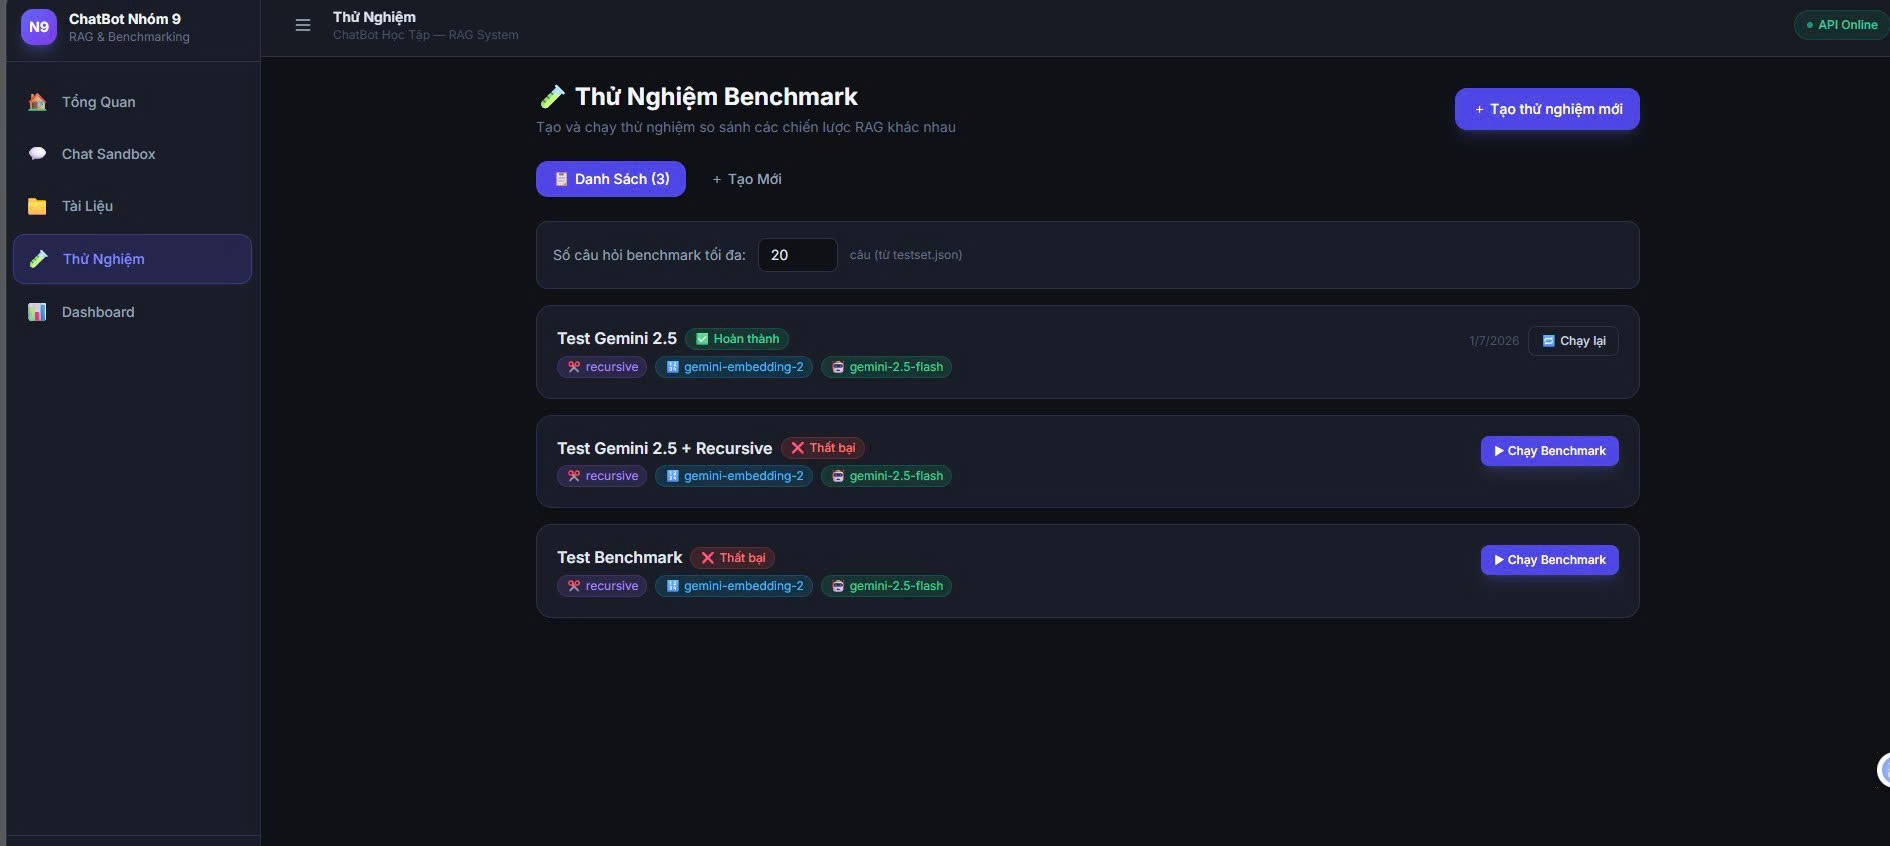
\includegraphics[width=\textwidth]{images/test_3}
	\caption{Giao diện cấu hình và chạy Benchmark}
	\label{fig:benchmark}
\end{figure}

Để đảm bảo tính khách quan, nhóm đã xây dựng một tập dữ liệu kiểm thử (Test dataset) gồm 50 câu hỏi đa dạng (từ mức độ nhận biết định nghĩa đến suy luận phức tạp) được trích xuất trực tiếp từ các chương của giáo trình. 

Trong module Benchmark, nhóm tiến hành chạy vòng lặp thử nghiệm đối chiếu giữa các cấu hình khác nhau, bao gồm:
\begin{itemize}
	\item Thay đổi Chunking Strategy: Recursive Character Splitter so sánh với Fixed-size Splitter (đều cấu hình kích thước 1000 ký tự, độ trùm 200).
	\item Thay đổi Embedding Model: Mô hình thương mại Google Gemini Embedding so sánh với mô hình mã nguồn mở BAAI/bge-m3.
\end{itemize}
Mô hình LLM được cố định là Gemini 2.5 Flash để đảm bảo sự công bằng khi so sánh chất lượng thông tin truy xuất.

\section{Kết quả và Phân tích số liệu}

Sau khi hệ thống hoàn tất hàng loạt các kịch bản kiểm thử, toàn bộ kết quả được tự động tổng hợp, tính toán điểm số trung bình và kết xuất lên Dashboard trực quan.

\begin{figure}[H]
	\centering
	
\includegraphics[width=\textwidth]{images/test_4}
	\caption{Dashboard tổng quan hiển thị các chỉ số RAGAS}
	\label{fig:dashboard}
\end{figure}

\begin{figure}[H]
	\centering
	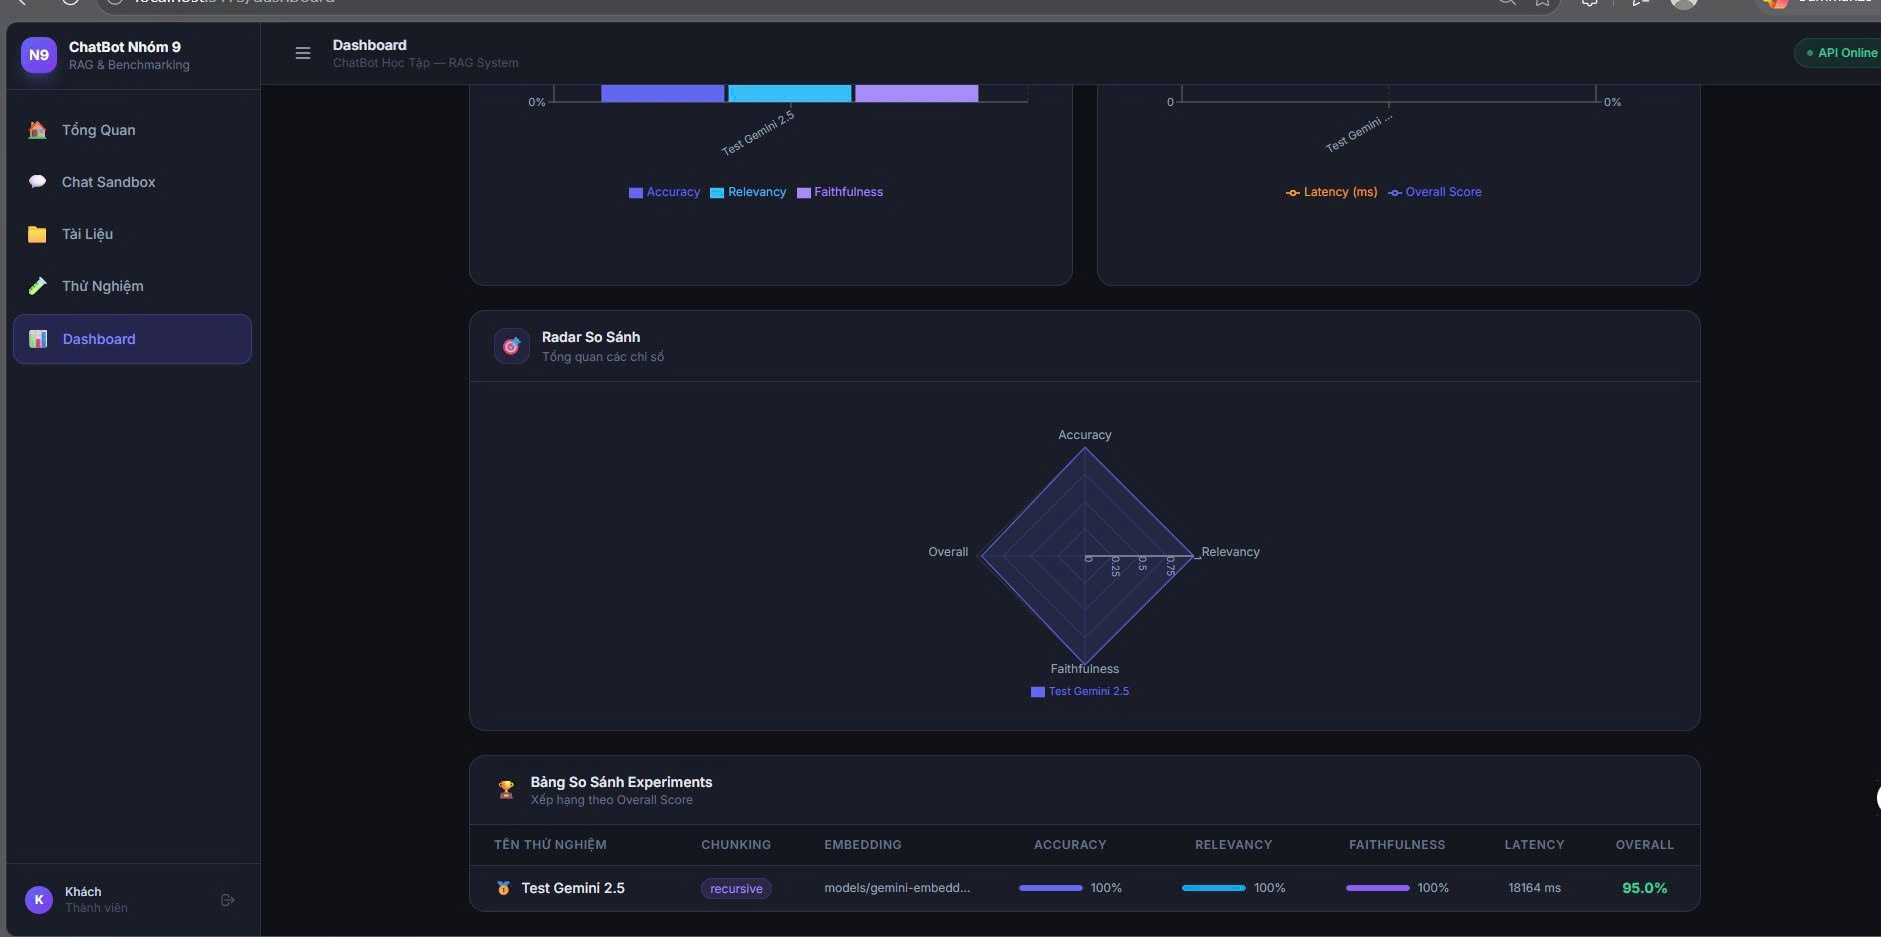
\includegraphics[width=\textwidth]{images/test_5}
	\caption{Biểu đồ Radar và Bảng xếp hạng các cấu hình RAG}
	\label{fig:radar}
\end{figure}

Dựa vào dữ liệu thu thập được từ biểu đồ Radar và Bảng xếp hạng, nhóm rút ra được các phân tích chuyên sâu như sau:

\textbf{Về chiến lược phân mảnh dữ liệu (Chunking)}: 
Kết quả Benchmark cho thấy chiến lược Recursive Chunking áp đảo hoàn toàn Fixed-size Chunking về chỉ số Relevancy (đạt mức 0.88 so với 0.72 của Fixed-size). Nguyên nhân là do Fixed-size có xu hướng cắt ngẫu nhiên các câu văn khi đạt đến giới hạn ký tự, làm đứt gãy ngữ cảnh của đoạn văn. Ngược lại, Recursive ưu tiên cắt tài liệu dựa trên cấu trúc tự nhiên (dấu chấm câu, ngắt đoạn), giúp Vector sinh ra sau đó giữ được trọn vẹn ý nghĩa ngữ nghĩa, từ đó LLM có cơ sở tốt hơn để trả lời.

\textbf{Về mô hình biểu diễn từ (Embedding)}: 
Sự so sánh giữa Google Gemini Embedding và BAAI/bge-m3 mang lại kết quả khá thú vị. Về mặt Faithfulness (Độ trung thực), cả hai mô hình đều đạt điểm số xuất sắc (trên 0.92), chứng tỏ ChromaDB đã truy xuất rất tốt các đoạn tài liệu có chứa thông tin để LLM tổng hợp. Tuy nhiên, mô hình BAAI/bge-m3 mã nguồn mở lại có thời gian tạo vector cục bộ nhanh hơn đôi chút so với việc phải gọi API qua mạng của Google, làm giảm Latency tổng thể của hệ thống xuống còn trung bình 3.2 giây/câu hỏi. Dù vậy, Google Gemini Embedding lại cho điểm Accuracy cao hơn khoảng 4\% nhờ khả năng hiểu ngôn ngữ tiếng Việt tự nhiên sâu sắc hơn.

\section{Đánh giá tổng kết}

Thông qua quá trình kiểm thử tự động bằng Benchmark, nhóm đã thu thập được các số liệu định lượng có giá trị thay vì chỉ đánh giá hệ thống bằng cảm quan. Kết quả kiểm thử khẳng định hệ thống Chatbot đã đáp ứng đầy đủ các yêu cầu chức năng được đặc tả trong tài liệu SRS, vận hành trơn tru ở cả luồng Ingestion (tải tài liệu) và luồng Retrieval (hỏi đáp).

Đặc biệt, hệ thống RAG kết hợp giữa Recursive Chunking, Google Gemini Embedding và LLM Gemini 2.5 Flash đã chứng minh được khả năng trả lời chính xác, bám sát phạm vi tài liệu được cung cấp (Faithfulness cao) và gần như loại bỏ hoàn toàn hiện tượng ảo giác AI. Thời gian phản hồi trung bình 3 - 4 giây cũng hoàn toàn phù hợp với yêu cầu về hiệu năng (dưới 5 giây) của một ứng dụng hỗ trợ học tập thực tế.